\section{Hidden Markov Model}

\begin{frame}Hidden Markov Model
\begin{figure}
\centering
	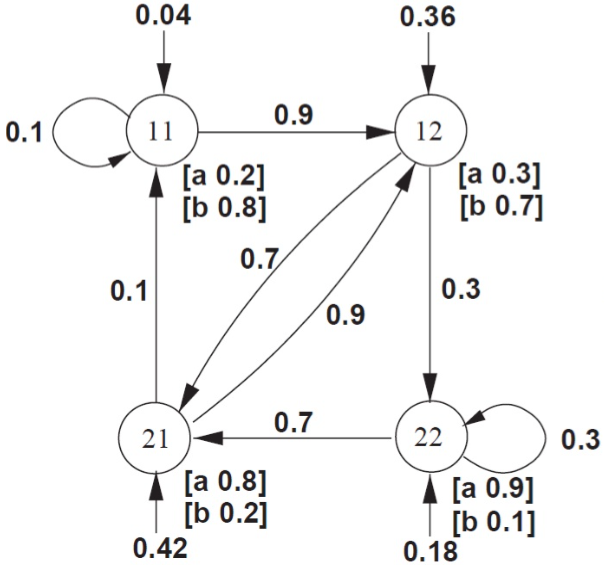
\includegraphics[scale=0.28]{./content/hmm}
	\caption{PAutomaC: a PFA/HMM Learning Competition, Sicco Verwer et al., 2012}
\end{figure}
\end{frame}


\begin{frame}Hidden Markov Model - Urn and Ball
\begin{figure}
\centering
	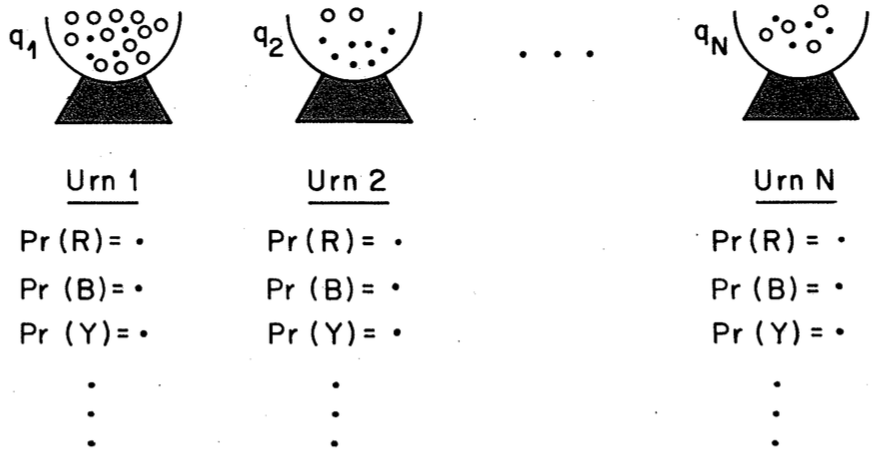
\includegraphics[scale=0.28]{./content/urn}
	\caption{An Introduction to Hidden Markov Models, L. R. Rabiner B. H. juang, 1986}
\end{figure}
\end{frame}


\begin{frame}Hidden Markov Model
	\begin{itemize}
		\item $T$ = length of observation sequence
		\item $N$ = number of states in the model
		\item $M$ = number of observation symbols
		\item $Q$ = \{$q_1, q_2,...,q_N$\}, states
		\item $V$ = \{$v_1, v_2,...,v_M$\}, \\
		observation symbols
		\item $A$ = \{$a_{ij}$\}, $a_{ij}$ = $Pr(q_j$, at $t + 1 | q_i$ at $t)$, \\
		state transition probability distribution
		\item $B$ = \{$b_j(k)$\}, $b_j(k)$ = $Pr(v_k$ at $t  | q_j$ at $t)$, \\
		observation symbol probability distribution
		\item $\pi$ = \{$\pi_i$\}, $\pi_i$ = $Pr(q_i$ at $t = 1)$, \\
		initial state distribution
		\item $\lambda$ = ($A$, $B$, $\pi$), the HMM
	\end{itemize}
	
	\begin{tikzpicture}[remember picture,overlay]  
      \node [xshift=-2.2cm,yshift=-3cm] at (current page.north east)
    {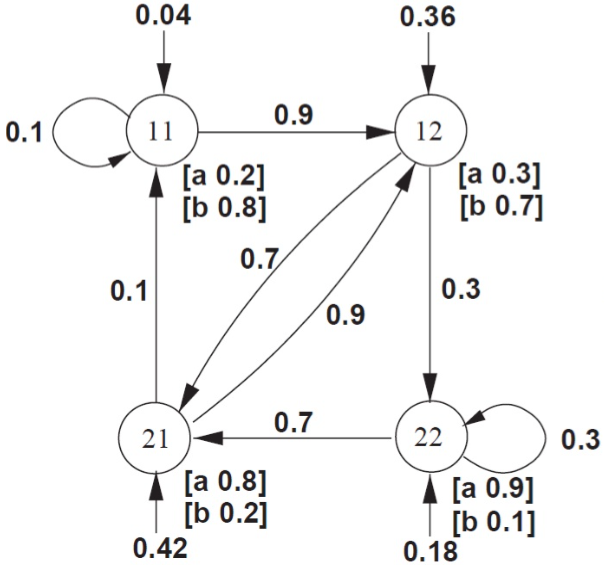
\includegraphics[scale=0.2]{./content/hmm}};
	\end{tikzpicture}		
\end{frame}